\chapter{Hopcroft's algorithm}

\subsection{algorithm}

Member function min\_Hopcroft implements Hopcroft's $n\log n$ minimization algorithm, as presented in [\cite{WATSON94b}, Algorithm 4.8].

The combination of the out-transitions of all of the States is stored in a
\textbf{CRSet $C$}. 

Set \text{$L$} from the abstract algorithm is implemented as a mapping from States to int (an array of int is used). 

Array $L$ should be interpreted as follows: if State q a representative,
then the following pairs still require processing (are still in abstract set L):
$$([q], C_0),\cdots, ([q], C_{L(q)-1}) $$

The remaining pairs do not require processing:
$$([q], C_{L[q])}),\cdots, ([q], C_{|C|-1}) $$

This implementation facilitates quick scanning of $L$ for the next valid State-CharRange pair.

\begin{algorithm}  
	\caption{Hopcroft's minimization algorithm}  \label{alg:hopcroft}
	\begin{algorithmic}[1] %每行显示行号  
		\Require $\mathcal{A}=(Q,i,F)$  
		\Ensure The equivalence classes of $Q$  
		\State $\hat{P} \gets \{F,F^c \}$  \qquad\qquad $\triangleright$ The initial partition
		\State $W\gets \emptyset$  \qquad\qquad $\triangleright$ The waiting set
		\ForAll {$a\in A$}
		\State $ADD((min(F,F^c),a),W)$ \qquad\qquad $\triangleright$ initialization of the waiting set
		\EndFor
		\While {$W\ne\emptyset$}
		\State $(W,a)\gets TakeSome(W)$ \qquad\qquad $\triangleright$ Take and remove some splitter
		\ForAll {$P\in \hat{P}$} which is split by $(W,a)$
		\State $P^{\prime},P^{\prime\prime}\gets (W,a)|P$ \qquad\qquad $\triangleright$ Compute the split
		\State Replace $P$ by $P^\prime$ and $P^{\prime\prime}$ in $\hat{P}$ \qquad\qquad $\triangleright$ Refine the partition
		\EndFor 
		\ForAll {$b\in A$}  \qquad\qquad $\triangleright$ Update the waiting set
		\If {$(P,b)\in W$}
		\State Replace $(P,b)$ by $(P^\prime,b)$ and $(P^{\prime\prime})$ in $W$
		\Else
		\State $ADD((min(P^\prime,P^{\prime\prime}),b),W)$
		\EndIf  
		\EndFor
		\EndWhile
	\end{algorithmic}
\end{algorithm}

\subsection{Example}

\begin{figure} \centering 
	\subfigure[DFA] { \label{fig:a1} 
		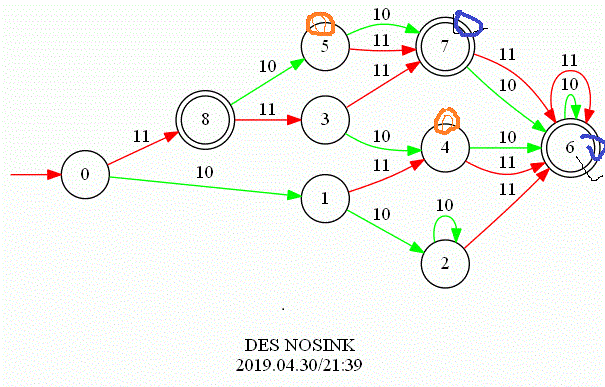
\includegraphics[width=0.4\columnwidth] {NOSINK} 
	} 
	\subfigure[mini-DFA] { \label{fig:b2} 
		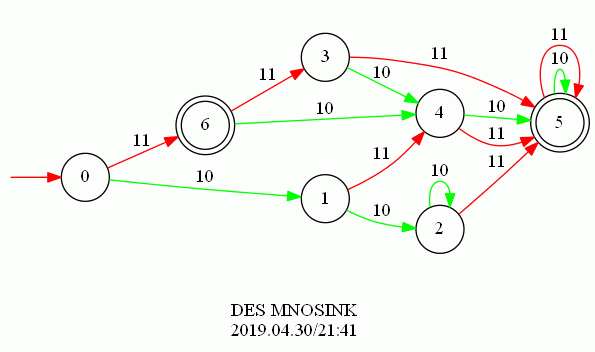
\includegraphics[width=0.4\columnwidth] {MNOSINK} 
	} 
	\caption{ example minimization } 
	\label{fig:mini-ex} 
\end{figure}



\begin{lstlisting}

CRSet C;  // the out labels of State's:{ 'a'  'b' }
int L[|Q|]: // the index of L = q: 对应等价类[q]; L[q]表示正在处理[q]对应的字符在C中的index,
0 1 2 3 4 5 6 7 8
0 0 0 0 0 0 0 0 0

Initialize partitions, E_0:
{ 0  1  2  3  4  5 }
{ 6  7  8 }

Initialize L repr{F}:  { 6 }
L:
0 1 2 3 4 5 6 7 8
0 0 0 0 0 0 2 0 0

--- while each [q], (split [p] w.r.t ([q],a))
L:
0 1 2 3 4 5 6 7 8
0 0 0 0 0 0 2 0 0

Pick one [q] in L, Processing [q]= index of L = [6],'b'
current all partitions:
{ 0  1  2  3  4  5 }
{ 6  7  8 }

=== for each [p], (split [p] w.r.t (index of L)[6],'b')

===split[0] w.r.t (index of L)[6],'b')
before split, partitions:
{ 0  1  2  3  4  5 }
{ 6  7  8 }

new split of [0] is [1]
after split, partitions:
{ 0  2  3  4  5 }
{ 1 }
{ 6  7  8 }

before L:
0 1 2 3 4 5 6 7 8
0 0 0 0 0 0 1 0 0

p and r are the new representatives. Now update L with the smallest of [0],[1]
using [r] = [1],L[r]=C.size();

affter L:
0 1 2 3 4 5 6 7 8
0 2 0 0 0 0 1 0 0

===split[6] w.r.t (index of L)[6],'b')
before split, partitions:
{ 0  2  3  4  5 }
{ 1 }
{ 6  7  8 }

new split of [6] is [8]
after split, partitions:
{ 0  2  3  4  5 }
{ 1 }
{ 6  7 }
{ 8 }

before L:
0 1 2 3 4 5 6 7 8
0 2 0 0 0 0 1 0 0

p and r are the new representatives. Now update L with the smallest of [6],[8]
using [r] = [8],L[r]=C.size();

affter L:
0 1 2 3 4 5 6 7 8
0 2 0 0 0 0 1 0 2

--- while each [q], (split [p] w.r.t ([index of L]=[q],a))
L:
0 1 2 3 4 5 6 7 8
0 2 0 0 0 0 1 0 2
Pick one [q] in L, Processing [q]= index of L = [1],'b'
current all partitions(eq.classes) repr:
{ 0  1  6  8 }
current all partitions:
{ 0  2  3  4  5 }
{ 1 }
{ 6  7 }
{ 8 }

=== for each [p], (split [p] w.r.t (index of L)[1],'b')
===split[0] w.r.t (index of L)[1],'b')
before split, partitions:
StateEqRel
{ 0  2  3  4  5 }
{ 1 }
{ 6  7 }
{ 8 }

new split of [0] is [-1]
===split[1] w.r.t (index of L)[1],'b')
before split, partitions:
{ 0  2  3  4  5 }
{ 1 }
{ 6  7 }
{ 8 }

new split of [1] is [-1]
===split[6] w.r.t (index of L)[1],'b')
before split, partitions:
{ 0  2  3  4  5 }
{ 1 }
{ 6  7 }
{ 8 }

new split of [6] is [-1]
===split[8] w.r.t (index of L)[1],'b')
before split, partitions:
StateEqRel
{ 0  2  3  4  5 }
{ 1 }
{ 6  7 }
{ 8 }

new split of [8] is [-1]
--- while each [q], (split [p] w.r.t ([index of L]=[q],a))
L:
0 1 2 3 4 5 6 7 8
0 1 0 0 0 0 1 0 2
Pick one [q] in L, Processing [q]= index of L = [1],'a'
current all partitions(eq.classes) repr:
{ 0  1  6  8 }
current all partitions:
{ 0  2  3  4  5 }
{ 1 }
{ 6  7 }
{ 8 }

=== for each [p], (split [p] w.r.t (index of L)[1],'a')
===split[0] w.r.t (index of L)[1],'a')
before split, partitions:
{ 0  2  3  4  5 }
{ 1 }
{ 6  7 }
{ 8 }

new split of [0] is [2]
after split, partitions:
StateEqRel
{ 0 }
{ 1 }
{ 2  3  4  5 }
{ 6  7 }
{ 8 }

before L:
L:
0 1 2 3 4 5 6 7 8
0 0 0 0 0 0 1 0 2
p and r are the new representatives. Now update L with the smallest of [0],[2]
using [p] = [0],L[r]=L[p]; L[p]=C.size();
affter L:
L:
0 1 2 3 4 5 6 7 8
2 0 0 0 0 0 1 0 2
===split[1] w.r.t (index of L)[1],'a')
before split, partitions:
StateEqRel
{ 0 }
{ 1 }
{ 2  3  4  5 }
{ 6  7 }
{ 8 }

new split of [1] is [-1]
===split[6] w.r.t (index of L)[1],'a')
before split, partitions:
StateEqRel
{ 0 }
{ 1 }
{ 2  3  4  5 }
{ 6  7 }
{ 8 }

new split of [6] is [-1]
===split[8] w.r.t (index of L)[1],'a')
before split, partitions:
StateEqRel
{ 0 }
{ 1 }
{ 2  3  4  5 }
{ 6  7 }
{ 8 }

new split of [8] is [-1]
--- while each [q], (split [p] w.r.t ([index of L]=[q],a))
L:
0 1 2 3 4 5 6 7 8
2 0 0 0 0 0 1 0 2
Pick one [q] in L, Processing [q]= index of L = [0],'b'
current all partitions(eq.classes) repr:
{ 0  1  2  6  8 }
current all partitions:
StateEqRel
{ 0 }
{ 1 }
{ 2  3  4  5 }
{ 6  7 }
{ 8 }

=== for each [p], (split [p] w.r.t (index of L)[0],'b')
===split[0] w.r.t (index of L)[0],'b')
before split, partitions:
StateEqRel
{ 0 }
{ 1 }
{ 2  3  4  5 }
{ 6  7 }
{ 8 }

new split of [0] is [-1]
===split[1] w.r.t (index of L)[0],'b')
before split, partitions:
StateEqRel
{ 0 }
{ 1 }
{ 2  3  4  5 }
{ 6  7 }
{ 8 }

new split of [1] is [-1]
===split[2] w.r.t (index of L)[0],'b')
before split, partitions:
StateEqRel
{ 0 }
{ 1 }
{ 2  3  4  5 }
{ 6  7 }
{ 8 }

new split of [2] is [-1]
===split[6] w.r.t (index of L)[0],'b')
before split, partitions:
StateEqRel
{ 0 }
{ 1 }
{ 2  3  4  5 }
{ 6  7 }
{ 8 }

new split of [6] is [-1]
===split[8] w.r.t (index of L)[0],'b')
before split, partitions:
StateEqRel
{ 0 }
{ 1 }
{ 2  3  4  5 }
{ 6  7 }
{ 8 }

new split of [8] is [-1]
--- while each [q], (split [p] w.r.t ([index of L]=[q],a))
L:
0 1 2 3 4 5 6 7 8
1 0 0 0 0 0 1 0 2
Pick one [q] in L, Processing [q]= index of L = [0],'a'
current all partitions(eq.classes) repr:
{ 0  1  2  6  8 }
current all partitions:
StateEqRel
{ 0 }
{ 1 }
{ 2  3  4  5 }
{ 6  7 }
{ 8 }

=== for each [p], (split [p] w.r.t (index of L)[0],'a')
===split[0] w.r.t (index of L)[0],'a')
before split, partitions:
StateEqRel
{ 0 }
{ 1 }
{ 2  3  4  5 }
{ 6  7 }
{ 8 }

new split of [0] is [-1]
===split[1] w.r.t (index of L)[0],'a')
before split, partitions:
StateEqRel
{ 0 }
{ 1 }
{ 2  3  4  5 }
{ 6  7 }
{ 8 }

new split of [1] is [-1]
===split[2] w.r.t (index of L)[0],'a')
before split, partitions:
StateEqRel
{ 0 }
{ 1 }
{ 2  3  4  5 }
{ 6  7 }
{ 8 }

new split of [2] is [-1]
===split[6] w.r.t (index of L)[0],'a')
before split, partitions:
StateEqRel
{ 0 }
{ 1 }
{ 2  3  4  5 }
{ 6  7 }
{ 8 }

new split of [6] is [-1]
===split[8] w.r.t (index of L)[0],'a')
before split, partitions:
StateEqRel
{ 0 }
{ 1 }
{ 2  3  4  5 }
{ 6  7 }
{ 8 }

new split of [8] is [-1]
--- while each [q], (split [p] w.r.t ([index of L]=[q],a))
L:
0 1 2 3 4 5 6 7 8
0 0 0 0 0 0 1 0 2
Pick one [q] in L, Processing [q]= index of L = [6],'a'
current all partitions(eq.classes) repr:
{ 0  1  2  6  8 }
current all partitions:
StateEqRel
{ 0 }
{ 1 }
{ 2  3  4  5 }
{ 6  7 }
{ 8 }

=== for each [p], (split [p] w.r.t (index of L)[6],'a')
===split[0] w.r.t (index of L)[6],'a')
before split, partitions:
StateEqRel
{ 0 }
{ 1 }
{ 2  3  4  5 }
{ 6  7 }
{ 8 }

new split of [0] is [-1]
===split[1] w.r.t (index of L)[6],'a')
before split, partitions:
StateEqRel
{ 0 }
{ 1 }
{ 2  3  4  5 }
{ 6  7 }
{ 8 }

new split of [1] is [-1]
===split[2] w.r.t (index of L)[6],'a')
before split, partitions:
StateEqRel
{ 0 }
{ 1 }
{ 2  3  4  5 }
{ 6  7 }
{ 8 }

new split of [2] is [4]
after split, partitions:
StateEqRel
{ 0 }
{ 1 }
{ 2  3 }
{ 4  5 }
{ 6  7 }
{ 8 }

before L:
L:
0 1 2 3 4 5 6 7 8
0 0 0 0 0 0 0 0 2
p and r are the new representatives. Now update L with the smallest of [2],[4]
using [p] = [2],L[r]=L[p]; L[p]=C.size();
affter L:
L:
0 1 2 3 4 5 6 7 8
0 0 2 0 0 0 0 0 2
===split[6] w.r.t (index of L)[6],'a')
before split, partitions:
StateEqRel
{ 0 }
{ 1 }
{ 2  3 }
{ 4  5 }
{ 6  7 }
{ 8 }

new split of [6] is [-1]
===split[8] w.r.t (index of L)[6],'a')
before split, partitions:
StateEqRel
{ 0 }
{ 1 }
{ 2  3 }
{ 4  5 }
{ 6  7 }
{ 8 }

new split of [8] is [-1]
--- while each [q], (split [p] w.r.t ([index of L]=[q],a))
L:
0 1 2 3 4 5 6 7 8
0 0 2 0 0 0 0 0 2
Pick one [q] in L, Processing [q]= index of L = [2],'b'
current all partitions(eq.classes) repr:
{ 0  1  2  4  6  8 }
current all partitions:
StateEqRel
{ 0 }
{ 1 }
{ 2  3 }
{ 4  5 }
{ 6  7 }
{ 8 }

=== for each [p], (split [p] w.r.t (index of L)[2],'b')
===split[0] w.r.t (index of L)[2],'b')
before split, partitions:
StateEqRel
{ 0 }
{ 1 }
{ 2  3 }
{ 4  5 }
{ 6  7 }
{ 8 }

new split of [0] is [-1]
===split[1] w.r.t (index of L)[2],'b')
before split, partitions:
StateEqRel
{ 0 }
{ 1 }
{ 2  3 }
{ 4  5 }
{ 6  7 }
{ 8 }

new split of [1] is [-1]
===split[2] w.r.t (index of L)[2],'b')
before split, partitions:
StateEqRel
{ 0 }
{ 1 }
{ 2  3 }
{ 4  5 }
{ 6  7 }
{ 8 }

new split of [2] is [-1]
===split[4] w.r.t (index of L)[2],'b')
before split, partitions:
StateEqRel
{ 0 }
{ 1 }
{ 2  3 }
{ 4  5 }
{ 6  7 }
{ 8 }

new split of [4] is [-1]
===split[6] w.r.t (index of L)[2],'b')
before split, partitions:
StateEqRel
{ 0 }
{ 1 }
{ 2  3 }
{ 4  5 }
{ 6  7 }
{ 8 }

new split of [6] is [-1]
===split[8] w.r.t (index of L)[2],'b')
before split, partitions:
StateEqRel
{ 0 }
{ 1 }
{ 2  3 }
{ 4  5 }
{ 6  7 }
{ 8 }

new split of [8] is [-1]
--- while each [q], (split [p] w.r.t ([index of L]=[q],a))
L:
0 1 2 3 4 5 6 7 8
0 0 1 0 0 0 0 0 2
Pick one [q] in L, Processing [q]= index of L = [2],'a'
current all partitions(eq.classes) repr:
{ 0  1  2  4  6  8 }
current all partitions:
StateEqRel
{ 0 }
{ 1 }
{ 2  3 }
{ 4  5 }
{ 6  7 }
{ 8 }

=== for each [p], (split [p] w.r.t (index of L)[2],'a')
===split[0] w.r.t (index of L)[2],'a')
before split, partitions:
StateEqRel
{ 0 }
{ 1 }
{ 2  3 }
{ 4  5 }
{ 6  7 }
{ 8 }

new split of [0] is [-1]
===split[1] w.r.t (index of L)[2],'a')
before split, partitions:
StateEqRel
{ 0 }
{ 1 }
{ 2  3 }
{ 4  5 }
{ 6  7 }
{ 8 }

new split of [1] is [-1]
===split[2] w.r.t (index of L)[2],'a')
before split, partitions:
StateEqRel
{ 0 }
{ 1 }
{ 2  3 }
{ 4  5 }
{ 6  7 }
{ 8 }

new split of [2] is [3]
after split, partitions:
StateEqRel
{ 0 }
{ 1 }
{ 2 }
{ 3 }
{ 4  5 }
{ 6  7 }
{ 8 }

before L:
L:
0 1 2 3 4 5 6 7 8
0 0 0 0 0 0 0 0 2
p and r are the new representatives. Now update L with the smallest of [2],[3]
using [p] = [2],L[r]=L[p]; L[p]=C.size();
affter L:
L:
0 1 2 3 4 5 6 7 8
0 0 2 0 0 0 0 0 2
胡
===split[4] w.r.t (index of L)[2],'b')
before split, partitions:
StateEqRel
{ 0 }
{ 1 }
{ 2 }
{ 3 }
{ 4  5 }
{ 6  7 }
{ 8 }

new split of [4] is [-1]
===split[6] w.r.t (index of L)[2],'b')
before split, partitions:
StateEqRel
{ 0 }
{ 1 }
{ 2 }
{ 3 }
{ 4  5 }
{ 6  7 }
{ 8 }

new split of [6] is [-1]
===split[8] w.r.t (index of L)[2],'b')
before split, partitions:
StateEqRel
{ 0 }
{ 1 }
{ 2 }
{ 3 }
{ 4  5 }
{ 6  7 }
{ 8 }

new split of [8] is [-1]
--- while each [q], (split [p] w.r.t ([index of L]=[q],a))
L:
0 1 2 3 4 5 6 7 8
0 0 1 0 0 0 0 0 2
Pick one [q] in L, Processing [q]= index of L = [2],'a'
current all partitions(eq.classes) repr:
{ 0  1  2  3  4  6  8 }
current all partitions:
StateEqRel
{ 0 }
{ 1 }
{ 2 }
{ 3 }
{ 4  5 }
{ 6  7 }
{ 8 }

=== for each [p], (split [p] w.r.t (index of L)[2],'a')
===split[0] w.r.t (index of L)[2],'a')
before split, partitions:
StateEqRel
{ 0 }
{ 1 }
{ 2 }
{ 3 }
{ 4  5 }
{ 6  7 }
{ 8 }

new split of [0] is [-1]
===split[1] w.r.t (index of L)[2],'a')
before split, partitions:
StateEqRel
{ 0 }
{ 1 }
{ 2 }
{ 3 }
{ 4  5 }
{ 6  7 }
{ 8 }

new split of [1] is [-1]
===split[2] w.r.t (index of L)[2],'a')
before split, partitions:
StateEqRel
{ 0 }
{ 1 }
{ 2 }
{ 3 }
{ 4  5 }
{ 6  7 }
{ 8 }

new split of [2] is [-1]
===split[3] w.r.t (index of L)[2],'a')
before split, partitions:
StateEqRel
{ 0 }
{ 1 }
{ 2 }
{ 3 }
{ 4  5 }
{ 6  7 }
{ 8 }

new split of [3] is [-1]
===split[4] w.r.t (index of L)[2],'a')
before split, partitions:
StateEqRel
{ 0 }
{ 1 }
{ 2 }
{ 3 }
{ 4  5 }
{ 6  7 }
{ 8 }

new split of [4] is [-1]
===split[6] w.r.t (index of L)[2],'a')
before split, partitions:
StateEqRel
{ 0 }
{ 1 }
{ 2 }
{ 3 }
{ 4  5 }
{ 6  7 }
{ 8 }

new split of [6] is [-1]
===split[8] w.r.t (index of L)[2],'a')
before split, partitions:
StateEqRel
{ 0 }
{ 1 }
{ 2 }
{ 3 }
{ 4  5 }
{ 6  7 }
{ 8 }

new split of [8] is [-1]
--- while each [q], (split [p] w.r.t ([index of L]=[q],a))
L:
0 1 2 3 4 5 6 7 8
0 0 0 0 0 0 0 0 2
Pick one [q] in L, Processing [q]= index of L = [8],'b'
current all partitions(eq.classes) repr:
{ 0  1  2  3  4  6  8 }
current all partitions:
StateEqRel
{ 0 }
{ 1 }
{ 2 }
{ 3 }
{ 4  5 }
{ 6  7 }
{ 8 }

=== for each [p], (split [p] w.r.t (index of L)[8],'b')
===split[0] w.r.t (index of L)[8],'b')
before split, partitions:
StateEqRel
{ 0 }
{ 1 }
{ 2 }
{ 3 }
{ 4  5 }
{ 6  7 }
{ 8 }

new split of [0] is [-1]
===split[1] w.r.t (index of L)[8],'b')
before split, partitions:
StateEqRel
{ 0 }
{ 1 }
{ 2 }
{ 3 }
{ 4  5 }
{ 6  7 }
{ 8 }

new split of [1] is [-1]
===split[2] w.r.t (index of L)[8],'b')
before split, partitions:
StateEqRel
{ 0 }
{ 1 }
{ 2 }
{ 3 }
{ 4  5 }
{ 6  7 }
{ 8 }

new split of [2] is [-1]
===split[3] w.r.t (index of L)[8],'b')
before split, partitions:
StateEqRel
{ 0 }
{ 1 }
{ 2 }
{ 3 }
{ 4  5 }
{ 6  7 }
{ 8 }

new split of [3] is [-1]
===split[4] w.r.t (index of L)[8],'b')
before split, partitions:
StateEqRel
{ 0 }
{ 1 }
{ 2 }
{ 3 }
{ 4  5 }
{ 6  7 }
{ 8 }

new split of [4] is [-1]
===split[6] w.r.t (index of L)[8],'b')
before split, partitions:
StateEqRel
{ 0 }
{ 1 }
{ 2 }
{ 3 }
{ 4  5 }
{ 6  7 }
{ 8 }

new split of [6] is [-1]
===split[8] w.r.t (index of L)[8],'b')
before split, partitions:
StateEqRel
{ 0 }
{ 1 }
{ 2 }
{ 3 }
{ 4  5 }
{ 6  7 }
{ 8 }

new split of [8] is [-1]
--- while each [q], (split [p] w.r.t ([index of L]=[q],a))
L:
0 1 2 3 4 5 6 7 8
0 0 0 0 0 0 0 0 1
Pick one [q] in L, Processing [q]= index of L = [8],'a'
current all partitions(eq.classes) repr:
{ 0  1  2  3  4  6  8 }
current all partitions:
StateEqRel
{ 0 }
{ 1 }
{ 2 }
{ 3 }
{ 4  5 }
{ 6  7 }
{ 8 }

=== for each [p], (split [p] w.r.t (index of L)[8],'a')
===split[0] w.r.t (index of L)[8],'a')
before split, partitions:
StateEqRel
{ 0 }
{ 1 }
{ 2 }
{ 3 }
{ 4  5 }
{ 6  7 }
{ 8 }

new split of [0] is [-1]
===split[1] w.r.t (index of L)[8],'a')
before split, partitions:
StateEqRel
{ 0 }
{ 1 }
{ 2 }
{ 3 }
{ 4  5 }
{ 6  7 }
{ 8 }

new split of [1] is [-1]
===split[2] w.r.t (index of L)[8],'a')
before split, partitions:
StateEqRel
{ 0 }
{ 1 }
{ 2 }
{ 3 }
{ 4  5 }
{ 6  7 }
{ 8 }

new split of [2] is [-1]
===split[3] w.r.t (index of L)[8],'a')
before split, partitions:
StateEqRel
{ 0 }
{ 1 }
{ 2 }
{ 3 }
{ 4  5 }
{ 6  7 }
{ 8 }

new split of [3] is [-1]
===split[4] w.r.t (index of L)[8],'a')
before split, partitions:
StateEqRel
{ 0 }
{ 1 }
{ 2 }
{ 3 }
{ 4  5 }
{ 6  7 }
{ 8 }

new split of [4] is [-1]
===split[6] w.r.t (index of L)[8],'a')
before split, partitions:
StateEqRel
{ 0 }
{ 1 }
{ 2 }
{ 3 }
{ 4  5 }
{ 6  7 }
{ 8 }

new split of [6] is [-1]
===split[8] w.r.t (index of L)[8],'a')
before split, partitions:
StateEqRel
{ 0 }
{ 1 }
{ 2 }
{ 3 }
{ 4  5 }
{ 6  7 }
{ 8 }

new split of [8] is [-1]
--- while each [q], (split [p] w.r.t ([index of L]=[q],a))
L:
0 1 2 3 4 5 6 7 8
0 0 0 0 0 0 0 0 0
\end{lstlisting}

\section{Minimization by equivalence of states}



\begin{figure}[htbp]
	\begin{tikzpicture}[->,>=stealth',shorten >=1pt,auto,node distance=2cm, semithick]
	\tikzstyle{every state}=[minimum size=0.1mm]
	\node[initial,state] (p1)  {$1$};
	\node[state]         (p2) [right of=p1] {$2$};
	\node[state]         (p3) [right of=p2] {$3$};
	\node[state]         (p4) [right of=p3] {$4$};
	\node[state]         (p5) [right of=p4] {$5$};
	\node[state,accepting] (p6) [right of=p5] {$6$};
	\path
	(p1) edge [loop above] node {1} (p1)
	     edge [] node {0} (p2)
	(p2) edge [loop above] node {1} (p2)
	     edge [] node {0} (p3)
	(p3) edge [loop above] node {1} (p3)
		 edge [] node {0} (p4)
    (p4) edge [loop above] node {1} (p4)
         edge [] node {0} (p5)
    (p5) edge [loop above] node {1} (p5)
         edge [] node {0} (p6)
    (p6) edge [loop above] node {0,1} (p6)
	;
	\end{tikzpicture}
	\caption{Minimizing example} \label{fig:mini-ex1}
\end{figure}



\begin{figure} [htbp]
	\{a,b\},\{d,e\}is not equivalent states. \\
	Sets of equivalent states: \{a,c\},\{b\},\{d\},\{e\}\\
	%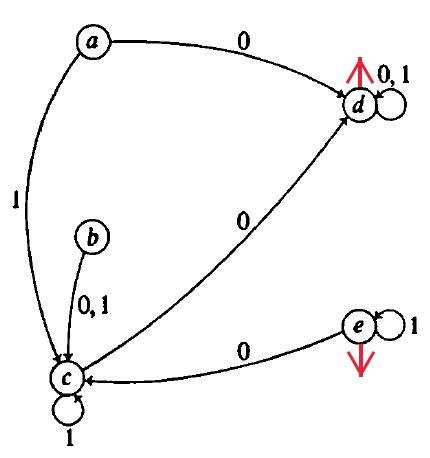
\includegraphics[scale=0.4] {mini-fa} 
	\begin{tikzpicture}[->,>=stealth',shorten >=1pt,auto,node distance=1.5cm, semithick]
	\tikzstyle{every state}=[minimum size=0.1mm]
	\node[state] (a) {$a$};
	\node[state,accepting] (d) [right of=a] {$d$};
	\node[state] (c) [below of=a] {$c$};
	\node[state] (b) [left of=c] {$b$};
	\node[state,accepting] (e) [right of=c] {$e$};
	\path
	(d) edge [loop above] node {$0,1$} (d)
	(c) edge [loop below] node {$1$} (c)
	(e) edge [loop below] node {$1$} (e)
	(a) edge [] node {$0$} (d)
	(a) edge [swap] node {$1$} (c)
	(b) edge [swap] node {$0,1$} (c)
	(e) edge [] node {$0$} (c)
	(c) edge [] node {$0$} (d)
	;
	\end{tikzpicture}
	\caption{Finite state automaton}
	\label{fig:mini-ex2}
\end{figure}




%%%%%%%%%%%%%%%%%%%%%%%%%%%%%%%%%%%%%%%%%%%%%%%%%%
\begin{thebibliography}{99}
		\bibitem[Hopcroft2008]{Hopcroft2008}
	John E. Hopcroft,Rajeev Motwani,Jeffrey D. Ullman著,孙家骕等译,\textit{自动机理论、语言和计算机导论},Third Edition, 机械工业出版社,2008.7
	
	\bibitem[WATSON93a]{WATSON93a}
	WATSON, B. W. \textit{A taxonomy of finite automata construction algorithms}, Computing Science Note 93/43, Eindhoven University of Technology, The Netherlands, 1993. Available by ftp from ftp.win.tue.nl in pub/techreports/pi.
	
	\bibitem[WATSON93b]{WATSON93b}
	WATSON, B. W. \textit{A taxonomy of finite automata minimization algorithms}, Computing Science Note 93/44, Eindhoven University of Technology, The Netherlands, 1993. Available by ftp from ftp.win.tue.nl in pub/techreports/pi.
	
	\bibitem[WATSON94a]{WATSON94a}
	WATSON, B. W. \textit{An introduction to the FIRE engine: A C++ toolkit for FInite automata and Regular Expressions}, Computing Science Note 94/21, Eindhoven University of Technology, The Netherlands, 1994. Available by ftp from ftp.win.tue.nl in pub/techreports/pi
	
	\bibitem[WATSON94b]{WATSON94b}
	WATSON, B.W. \textit{The design. and implementation of the FIRE engine:	A C++ toolkit for FInite automata and Regular Expressions}, Computing Science Note 94/22, Eindhoven University of Technology, The Netherlands, 1994. Available by ftp from ftp.win.tue.nl in pub/techreports/pi.
	
	\bibitem[Chrison2007]{Chrison2007}
	Christos G. Cassandras and St$\acute{e}$phane Lafortune, \textit{Introduction to Discrete Event Systems},Second Edition,New York,Springer,2007
	
	\bibitem[Wonham2018]{Wonham2018}
	W. M. Wonham and Kai Cai,\textit{Supervisory Control of Discrete-Event Systems}, Revised 2018.01.01
	
	\bibitem[Jean2018]{Jean2018}
	Jean-$\acute{E}$ric Pin, \textit{Mathematical Foundations of Automata Theory},Version of June 15,2018
	
	\bibitem[蒋宗礼2013]{蒋宗礼2013}
	蒋宗礼,姜守旭, \textit{形式语言与自动机理论(第3 版)}, 清华大学出版社,2013.05
	
	
	\bibitem[Lipschutz2007]{Lipschutz2007}
	S. Lipschutz and M. L. Lipson, \textit{Schaum's Outline of Theory and Problems of Discrete Mathematics}, Third Edition, New York: McGraw-Hill, 2007.
	
	\bibitem[Rosen2007]{Rosen2007}
	K. H. Rosen, \textit{Discrete Mathematics and Its Applications}, Seventh Edition, New York: McGraw-Hill, 2007.
	
	\bibitem[R.Su and Wonham2004]{R.Su and Wonham2004}
	R. Su and W. M. Wonham, \textit{Supervisor reduction for discrete-event systems}, Discrete Event Dyn. Syst., vol. 14, no. 1, pp. 31–53, Jan. 2004.
	
	\bibitem[Hopcroft71]{Hopcroft71}
	Hopcroft, J.E. \textit{An n log n algorithm for minimizing states in a finite automaton}, in The Theory of Machines and Computations (Z. Kohavi, ed.), pp.180-196, Academic Press, New York, 1971.
	
	\bibitem[Gries73]{Gries73}
	Gries, D. \textit{Describing an Algorithm by Hopcroft}, Acta Inf. 2:97 109, 173. $\copyright$ by Springer-Verlag 1973
	
	\bibitem[Knuutila2001]{Knuutila2001}
	Knuutila, T. \textit{Re-describing an Algorithm by Hopcroft}. Theoret. Computer Science 250 (2001) 333--363.
	
	\bibitem[Ratnesh95]{Ratnesh95}
	Ratnesh Kumar, \textit{Modeling and Control of Logical Discrete Event Systems}, $\copyright$ 1995 by Springer Science+Business Media New York.
	
	\bibitem[Jean2011]{Jean2011}
	Jean Berstel, Luc Boasson, Olivier Carton, Isabelle Fagnot
	, \textit{Minimization of automata}, Universit$\acute{e}$ Paris-Est Marne-la-Vall$\acute{e}$e 2010 Mathematics Subject Classification: 68Q45, 2011.
	
	\bibitem[Kenneth2012]{Kenneth2012}
	Kenneth H. Rosen著,徐六通译, \textit{离散数学及其应用Discrete Mathematics and Its Applications},seventh Edition, 2012, 机械工业出版社, 北京, 2014.
	
\end{thebibliography}
